% Options for packages loaded elsewhere
\PassOptionsToPackage{unicode}{hyperref}
\PassOptionsToPackage{hyphens}{url}
%
\documentclass[
  10pt,
]{article}
\usepackage{amsmath,amssymb}
\usepackage{iftex}
\ifPDFTeX
  \usepackage[T1]{fontenc}
  \usepackage[utf8]{inputenc}
  \usepackage{textcomp} % provide euro and other symbols
\else % if luatex or xetex
  \usepackage{unicode-math} % this also loads fontspec
  \defaultfontfeatures{Scale=MatchLowercase}
  \defaultfontfeatures[\rmfamily]{Ligatures=TeX,Scale=1}
\fi
\usepackage{lmodern}
\ifPDFTeX\else
  % xetex/luatex font selection
\fi
% Use upquote if available, for straight quotes in verbatim environments
\IfFileExists{upquote.sty}{\usepackage{upquote}}{}
\IfFileExists{microtype.sty}{% use microtype if available
  \usepackage[]{microtype}
  \UseMicrotypeSet[protrusion]{basicmath} % disable protrusion for tt fonts
}{}
\makeatletter
\@ifundefined{KOMAClassName}{% if non-KOMA class
  \IfFileExists{parskip.sty}{%
    \usepackage{parskip}
  }{% else
    \setlength{\parindent}{0pt}
    \setlength{\parskip}{6pt plus 2pt minus 1pt}}
}{% if KOMA class
  \KOMAoptions{parskip=half}}
\makeatother
\usepackage{xcolor}
\usepackage[margin=0.7in]{geometry}
\usepackage{longtable,booktabs,array}
\usepackage{calc} % for calculating minipage widths
% Correct order of tables after \paragraph or \subparagraph
\usepackage{etoolbox}
\makeatletter
\patchcmd\longtable{\par}{\if@noskipsec\mbox{}\fi\par}{}{}
\makeatother
% Allow footnotes in longtable head/foot
\IfFileExists{footnotehyper.sty}{\usepackage{footnotehyper}}{\usepackage{footnote}}
\makesavenoteenv{longtable}
\usepackage{graphicx}
\makeatletter
\def\maxwidth{\ifdim\Gin@nat@width>\linewidth\linewidth\else\Gin@nat@width\fi}
\def\maxheight{\ifdim\Gin@nat@height>\textheight\textheight\else\Gin@nat@height\fi}
\makeatother
% Scale images if necessary, so that they will not overflow the page
% margins by default, and it is still possible to overwrite the defaults
% using explicit options in \includegraphics[width, height, ...]{}
\setkeys{Gin}{width=\maxwidth,height=\maxheight,keepaspectratio}
% Set default figure placement to htbp
\makeatletter
\def\fps@figure{htbp}
\makeatother
\setlength{\emergencystretch}{3em} % prevent overfull lines
\providecommand{\tightlist}{%
  \setlength{\itemsep}{0pt}\setlength{\parskip}{0pt}}
\setcounter{secnumdepth}{-\maxdimen} % remove section numbering
\ifLuaTeX
  \usepackage{selnolig}  % disable illegal ligatures
\fi
\usepackage{bookmark}
\IfFileExists{xurl.sty}{\usepackage{xurl}}{} % add URL line breaks if available
\urlstyle{same}
\hypersetup{
  hidelinks,
  pdfcreator={LaTeX via pandoc}}

\author{}
\date{}

\begin{document}

\section{Exact normalized scaling and full closure under a target-row
change}\label{exact-normalized-scaling-and-full-closure-under-a-target-row-change}

2026-11-14. Source \texttt{85c57a726a644a6d2138a5c97785ab1119a06aff}.
All claims unsigned {[}pcc:unverified{]}.

The normalized target row has an exact inverse-pair pole-scaling law.
More decisively, the actual change of rows preserves the full iterated
degree-budgeted closure whenever the budget admits both input families.
This is a statement about the actual symbolic coefficient algebra, not
just equality of finite-field solution sets. It isolates what this
normalization can change and redirects the search for a closure
improvement beyond a constant row basis {[}pcc:unverified{]}.

Central claims: normalized scaling \texttt{PCC-20261114-46dee9}, generic
full closure \texttt{PCC-20261114-5f67e7}, actual normalized row
\texttt{PCC-20261114-044d98}, actual full closure
\texttt{PCC-20261114-d07690}. Gate/build receipt
\texttt{PCC-20261114-f6eb11}.
\href{../lean/NormTargetGrading.lean}{Scaling source},
\href{../lean/NormRowClosure.lean}{closure source},
\href{../TARGET_GRADING_PROTOCOL.md}{prospective contract},
\href{../target-grading-evidence/claim-pins.json}{exact proof map},
\href{closure.dot}{editable diagram}, \href{closure.svg}{SVG},
\href{report.pdf}{PDF}.

\begin{figure}
\centering
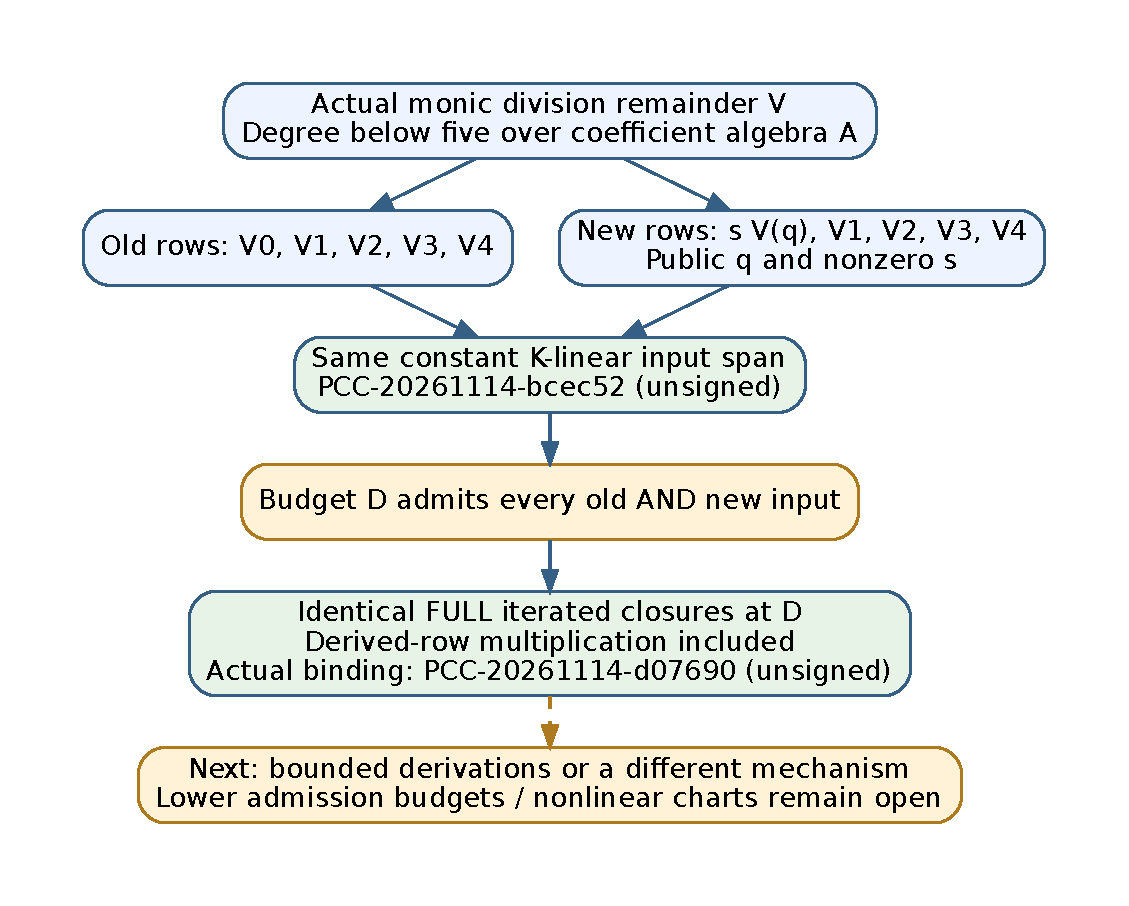
\includegraphics[width=0.88\textwidth,height=\textheight]{closure.pdf}
\caption{The exact row transformation preserves the full closure once
both sets of inputs are admitted. The lower-budget and nonlinear routes
remain separate. Evidence unsigned.}
\end{figure}

\subsection{Exact normalized scaling}\label{exact-normalized-scaling}

Keep the actual monic norm quotient, actual Dickson dividend and actual
membership quotient from the previous component. Write \(d=2^{n+1}\) and
\(R_e\) for the membership remainder. Its normalized target row is

\[
T_e=e^{d-3}(M_n(2)(r)-c)
 -(c_0+c_1e^2r)J_e Q_e(e^2r),
\]

where \(Q_e\) is the computed monic quotient and

\[
J_e=2za_1+4e^2zra_2+6e^4zr^2
 -e(3r^2+a)(c_0+c_1e^2r)-2e^3z^2c_1.
\]

The prior actual division gives \(R_e(e^2r)=e^3T_e\). Parameter one is
exactly \(T_1=R_1(r)\). Evaluating the full-remainder transport at the
scaled target and cancelling only the explicit nonzero factor gives

\[
e^{d-3}T_1(a_1l^4,a_2l^2,c_0l^3,c_1l)
 =T_e(a_1,a_2,c_0,c_1),\qquad el=1.
\]

The curve premise \(z^2=r^3+ar+b\) and \(d\ge3\) remain explicit. The
identity holds at every stated depth over a field; it is not yet an
identification with a formal multivariate weighted homogeneous
component. Thus weight29 at depth4 remains a candidate upper bound, not
an established exact degree {[}pcc:unverified{]}.

\subsection{Full closure, rather than static input
multiples}\label{full-closure-rather-than-static-input-multiples}

Let \(A\) be a commutative algebra over a field \(K\), and let
\(\delta:A\to\mathbb N\) be an explicit degree function. The inductive
closure at budget \(D\) allows:

\begin{enumerate}
\def\labelenumi{\arabic{enumi}.}
\tightlist
\item
  an input \(f\) only when \(\delta(f)\le D\);
\item
  zero, addition and multiplication by a scalar in \(K\);
\item
  multiplication of \textbf{any already derived row} \(f\) by \(a\in A\)
  when \(\delta(a)+\delta(f)\le D\).
\end{enumerate}

These are the literal full-closure rules of the existing ML source,
rebuilt at this study's pinned toolchain. Ordinary total degree and
weighted total degree can each instantiate the explicit function. No
static Macaulay-space surrogate, available GB or normal-form oracle is
assumed {[}pcc:unverified{]}.

If input sets \(F,G\) have equal \(K\)-linear spans and every member of
both sets is admitted at \(D\), their complete closures at \(D\)
coincide. The proof first puts each input span in the opposite closure,
then transports every derivation, including multiplication of derived
rows. It needs no theorem about the size of a solution set
{[}pcc:unverified{]}.

\subsection{Binding to the actual normalized target
row}\label{binding-to-the-actual-normalized-target-row}

For an actual degree-below-five remainder \(V\in A[X]\), public
\(q\in K\) and public \(s\ne0\), the old inputs are its five
coefficients. The new inputs are \(sV(q)\) and coefficients1 through4.
Polynomial evaluation gives

\[
V(q)=V_0+qV_1+q^2V_2+q^3V_3+q^4V_4.
\]

This is an invertible constant row transformation: solve for \(V_0\)
using \(s^{-1}\). Hence the generator spans agree. For the actual
membership remainder the degree guard follows from monic norm/support
division; \(q=e^2r\) and \(s=(e^3)^{-1}\) give exactly \(T_e\). Public
curve and parameter values are mapped into \(A\) by its algebra map,
while the retained coefficients remain arbitrary elements of \(A\). In
particular, \(A\) may be the multivariate polynomial ring in those
coefficients: this is a symbolic identity, not equality after sampling
{[}pcc:unverified{]}.

Consequently, once both original and normalized input families fit
\(D\), the same rows are derivable in their full closures. The theorem
keeps both admission hypotheses explicit; it does not assert a numerical
admission threshold for an unproved weighted grading
{[}pcc:unverified{]}.

\subsection{What the test decides}\label{what-the-test-decides}

Constant row recombination alone cannot lower the full closure above
that input-admission threshold. This tests the proposed mechanism before
using a degree fall as evidence of a faster solver. It leaves open
effects below the threshold, implementation changes, different degree
functions, nonlinear charts, different factor bases and other
non-generic algorithms. It does not show that the original closure is
large: the transformed row may still expose short derivations already
present in it. It is not a generic-group lower bound or a global
impossibility result {[}pcc:unverified{]}.

The exact transformation and scaling remain useful algebraic
information. A subsequent candidate needs to change something beyond
this constant input span, or supply actual bounded derivations and a
complete solver cost. The original nonscalar-origin/jet family still
needs its own faithful map; this norm normalization is not a map to that
family {[}pcc:unverified{]}.

\subsection{Sources, validation and retained
failures}\label{sources-validation-and-retained-failures}

Sources checked (KB): unavailable as previously documented, no unchanged
retry. The
\href{../target-grading-evidence/prior-search-receipt.json}{bounded
receipt} records three fallback queries and actual primary sources. Read
ML commit \texttt{8020e131a1a3806531d695b6bc7586473802dada}
\texttt{formal/ICFallDegrees/\{Closure,VariableClosure,FiniteQuotient,PointIdeal\}.lean}.
The finite-quotient result needs an available GB/reduced-ideal
subsystem; the point-ideal result needs budgeted coordinate derivations.
Neither discharges those premises from a small zero set. Prior
weighted-GB source review and Mathlib's weighted homogeneous definitions
remain relevant. This bounded review establishes no novelty or
exhaustive absence {[}pcc:unverified{]}.

Final normalized build002 and closure build005 exit0. There are15
authored theorem bindings. The whole-study gate audits369 declarations,
including the new generated \texttt{InClosure.brecOn}, and reports0
additional trusted uses, exit0. Standard foundations only. Exact
source/log hashes are in the
\href{../target-grading-evidence/gate-build-001.json}{gate receipt},
claim \texttt{PCC-20261114-f6eb11}; theorem claims are unsigned/default
not\_covered (exit2). Import-inclusive fresh replay exits0, including
both new modules; validation receipt PCC-20261114-6643d4 binds the exact
hashes {[}pcc:unverified{]}.

Retain normalized draft001's parameter-one wrapper error, closure
drafts001 through003's predicate, field, notation, recursive parameter
and coercion errors, and draft004's unnecessary tactic-sequencing
warning. The final source fixes these without changing statements,
suppressing checks or adding trusted axioms. No Rust/native mathematical
source changed and no prior native test was counted again. The inherited
canonical SHA256 clippy and benchrec diagnostics remain untouched
{[}pcc:unverified{]}.

No fixture, unknown-root, F4/msolve, paid/cloud/attack or timing
experiment was attempted. The earlier native fixture remains1 planned,0
attempted, 0 completed,0 excluded,1 admission-blocked by checkpoint
upload transport. Local Lean proof construction is separate. Complete
growing-family closure, an efficient public-input finder, extraction and
expected bit cost remain open {[}pcc:unverified{]}.

Global performance/curve/attack-route graphs are unchanged: this
component adds no measured speedup or group-transport edge. All previous
sources, evidence, claims and canonical ledger prefix are preserved. The
new visual records the exact mechanism and its scope
{[}pcc:unverified{]}.

\subsection{Exact proof map}\label{exact-proof-map}

All entries unsigned {[}pcc:unverified{]}. Declaration/context hashes
and source freeze are in claim-pins.json.

\begin{longtable}[]{@{}ll@{}}
\toprule\noalign{}
Declaration & Claim \\
\midrule\noalign{}
\endhead
\bottomrule\noalign{}
\endlastfoot
\texttt{NormTargetGrading.actualTargetFactor} &
\texttt{PCC-20261114-17b15a} \\
\texttt{NormTargetGrading.normalizedOne} &
\texttt{PCC-20261114-4f506d} \\
\texttt{NormTargetGrading.membershipOne} &
\texttt{PCC-20261114-d8ecad} \\
\texttt{NormTargetGrading.targetValueScale} &
\texttt{PCC-20261114-f41fe3} \\
\texttt{NormTargetGrading.normalizedScale} &
\texttt{PCC-20261114-46dee9} \\
\texttt{NormRowClosure.transport} & \texttt{PCC-20261114-7326e0} \\
\texttt{NormRowClosure.inputSpan} & \texttt{PCC-20261114-d0640f} \\
\texttt{NormRowClosure.closureSpanInvariant} &
\texttt{PCC-20261114-5f67e7} \\
\texttt{NormRowClosure.evaluationRows} & \texttt{PCC-20261114-a28623} \\
\texttt{NormRowClosure.rowsMembership} & \texttt{PCC-20261114-a2c68b} \\
\texttt{NormRowClosure.rowSpans} & \texttt{PCC-20261114-bcec52} \\
\texttt{NormRowClosure.rowClosure} & \texttt{PCC-20261114-1f8f28} \\
\texttt{NormRowClosure.actualMembershipWindow} &
\texttt{PCC-20261114-87bdd8} \\
\texttt{NormRowClosure.actualNormalizedRow} &
\texttt{PCC-20261114-044d98} \\
\texttt{NormRowClosure.actualRowClosure} &
\texttt{PCC-20261114-d07690} \\
\end{longtable}

\end{document}
